\problemname{Circular Shortcut}

% optionally define variables/limits for this problem
\newcommand{\maxd}{10^9}

After the practice session, Katrin and her team join the guided city tour of Karlsruhe,
where they learn all sorts of random fun facts about Karlsruhe.
It is well-known that the first email in Germany was received here (sent by Laura Breeden, MIT)
and that the bicycle was invented in Karlsruhe,
but did you know that the palace has exactly 365 windows -- one for each day of the year?
Or that there may (or may not) be an umbrella buried beneath the great pyramid in the city centre?

Later that evening, Katrin and her team find themselves in the western part of Karlsruhe,
and they have to hurry to the Dining Hall to make it in time for dinner!
They could take the direct route through the palace garden, which is a straight line.
But on such a pleasant evening, the palace garden is crowded with pedestrians and cyclists who might slow them down.
The alternative is to follow the \emph{Adenauerring},
a street forming a perfect half-circle between their current location and the intersection close to the Dining Hall,
and nothing will slow them down there.

\begin{figure}[h]
    \centering
    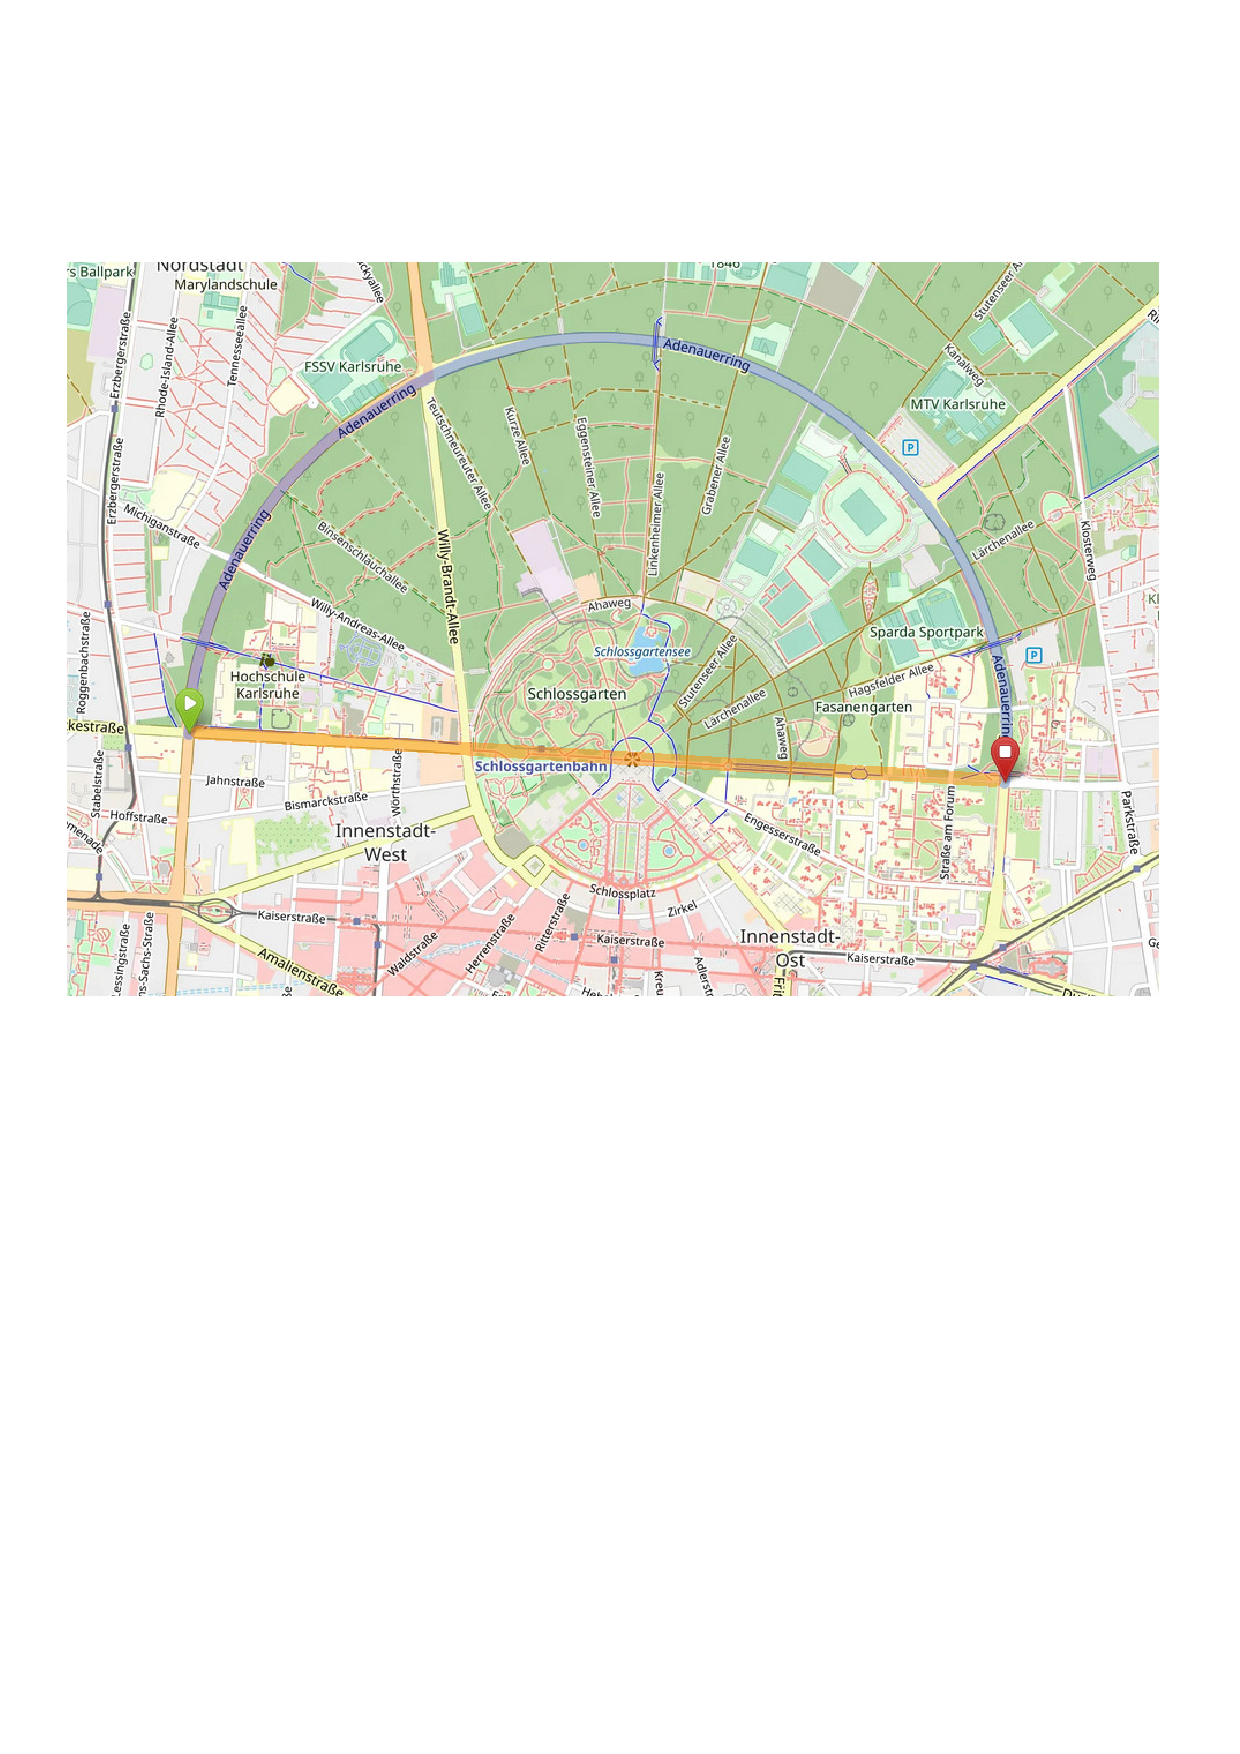
\includegraphics[width=0.45\textwidth]{map.pdf} \\
    \tiny Map data from \href{https://www.openstreetmap.org/copyright}{OpenStreetMap}
    \caption{The two possible paths from their current location to the
    intersection close to the Dining Hall. The blue semi-circular road is the
    Adenauerring, and the orange straight path in the middle is the route through the palace garden.}
    \label{fig:shortcut}
\end{figure}

% Given the length of the straight way through the palace garden in metres, how much longer is the route along the Adenauerring in metres?
Katrin and her team have arranged to meet up with their coach on the intersection close to the Dining Hall,
as shown in Figure~\ref{fig:shortcut}.
They would like to know: how much longer is the route along the Adenauerring?

\begin{Input}
    The input consists of:
    \begin{itemize}
        \item One line with an integer $d$ ($1\leq d\leq \maxd$),
            the length of the straight way through the palace garden, in metres.
    \end{itemize}
\end{Input}

\begin{Output}
    Output how much longer the route along the Adenauerring is, compared to going straight through the palace garden, in metres.

    Your answer should have an absolute or relative error of at most $10^{-9}$.
\end{Output}
